\documentclass[french, 12pt]{article}%


\usepackage[T1]{fontenc}
\usepackage[utf8]{inputenc}
\usepackage[french]{babel}

\usepackage{textcomp}

\usepackage[official]{eurosym}

\usepackage{appendix}
\usepackage{pdfpages}


%%%%%%%%%%%%%%%%%%%%%%%%%%%%%%%%%%%%%%%%%%%%%%%%%%%%%%%%%
\newcommand{\itemE}{\item[$\bullet$]}
\newcommand{\titreSeq}{Présentation de GIT}
\newcommand{\lycee}{Lycée de Brocéliande}
\newcommand{\classSeq}{CIEL2 }
\newcommand{\matiereSeq}{IR}      
\newcommand{\numSeq}{Cyber}
\newcommand{\numAct}{00}
\newcommand{\objSeance}{Comprendre le mécanisme de GIT}

\newcommand{\moySeq}{\begin{itemize}	
\itemE Machine Windows et Linux 

\end{itemize}}

\newcommand{\compSeq}{\begin{itemize}
\item  
\end{itemize}}
%%%%%%%%%%%%%%%%%%%%%%%%%%%%%%%%%%%%%%%%%%%%%%%%%%%%%%%%%%

%%%%%%%%%%%%%%%%%%%%%%%%%%%%%%%%%%%%%%%%%%%%%%%%%%%%%%%%
%%%%Algo
\usepackage[linesnumbered, french]{algorithm2e}
\SetKwFor{For}{Pour}{faire}{fin}
\SetKwFor{While}{Tant que}{faire}{fin}%
\SetKw{KwTo}{à}
\SetKw{KwPas}{par pas de}
\SetKw{KwRet}{Retourne}
\SetKwProg{Fn}{Fonction }{ arguments }{fin}
\SetKwRepeat{Repeat}{Répéter}{jusqu'à}%
\SetKwIF{If}{ElseIf}{Else}{Si}{alors}{Sinon si}{Sinon}{Fin}


\usepackage{listings} %%%%Présenration code source
\lstset{language=C++,
    %numbers=left,
    %stepnumber=1,
    showstringspaces=false,
    %tabsize=1,
    %breaklines=true,
    %breakatwhitespace=false,
    basicstyle=\footnotesize,
    keywordstyle=\color{blue}\footnotesize,
    stringstyle=\color{red}\footnotesize,
    commentstyle=\color{green}\footnotesize,
    morecomment=[l][\color{magenta}]{\#}
    }

%\usepackage[T1]{fontenc}
\lstdefinestyle{commande}{
  basicstyle=\ttfamily\footnotesize,
  keywordstyle=\color{blue},
  commentstyle=\color{gray},
  %numbers=left,
  %numberstyle=\tiny\color{gray},
  numbersep=5pt,
  breaklines=true,
  frame=single,
  backgroundcolor=\color{lightgray!10},
  %captionpos=b,
  %caption=\lstname   
    extendedchars=true,
    literate={é}{{\'e}}1
             {è}{{\`e}}1
             {à}{{\`a}}1
             {ç}{{\c{c}}}1
             {✔}{{\checkmark}}1,
}

% Margins
\topmargin=-0.45in
\evensidemargin=0in
\oddsidemargin=0in
\textwidth=6.5in
\textheight=9.0in
\headsep=0.25in 


\linespread{1.1} 
\usepackage{amsmath}%
\usepackage{amsfonts}%
\usepackage{amssymb}%
\usepackage{graphicx}
\usepackage{lastpage}
\usepackage{enumitem}

%\usepackage[T1]{fontenc}    
\usepackage{multirow}
\usepackage{lscape}
\usepackage[colorlinks = true,
            linkcolor = blue,
            urlcolor  = blue,
            citecolor = blue,
            anchorcolor = blue]{hyperref}
\usepackage{array}
\usepackage{mwe}
%-------------------------------------------
\newtheorem{theorem}{Theorem}
\newtheorem{summary}[theorem]{Summary}
\newenvironment{proof}[1][Proof]{\textbf{#1.} }{\ \rule{0.5em}{0.5em}}



\usepackage{xcolor}

\usepackage{colortbl}
\definecolor{vert_capet}{RGB}{191,255,191}	
\definecolor{bleu_snir}{RGB}{101,191,179}	
\setlength{\doublerulesep}{\arrayrulewidth}
%-------------------------------------------
%%%%%%%%%%%%%%%%%%%%%%%%%%%%%%%%%%%%%%%%%%%%%
\usepackage[framemethod=tikz]{mdframed}
\usepackage{tikz, xcolor, lipsum}
\makeatletter
\mdfsetup{skipabove=\topskip,skipbelow=\topskip}

\tikzset{titre_bleu_snir/.style =
	{draw=bleu_snir, line width=1.5pt, fill=white,
	rectangle, rounded corners, right,minimum height=2em}}
\newcommand{\titreencadre}{Titre}
\makeatletter
\mdfdefinestyle{encadrestyle}{%
	linewidth=1.5pt,roundcorner=5pt,linecolor=bleu_snir,
	apptotikzsetting={\tikzset{mdfbackground/.append style ={%
		fill=white}}},
	frametitlefont=\bfseries,
	singleextra={%
		\node[titre_bleu_snir,xshift=2em] at (P-|O) %
			{~\mdf@frametitlefont{\titreencadre}\hbox{~}};},
	firstextra={%
		\node[titre_bleu_snir,xshift=2em] at (P-|O) %
		{~\mdf@frametitlefont{\titreencadre}\hbox{~}};},
	}
\mdfdefinestyle{encadresanstitrestyle}{%
	linewidth=1.5pt,roundcorner=5pt,linecolor=bleu_snir
	apptotikzsetting={\tikzset{mdfbackground/.append style ={%
		fill=yellow!20}}},
	}

\newenvironment{encadre}[1]{\renewcommand{\titreencadre}{#1}
	\begin{mdframed}[style=encadrestyle]
	\vspace{0.5\baselineskip}
	}{%
	\end{mdframed}}

\newenvironment{encadresanstitre}{
	\begin{mdframed}[style=encadresanstitrestyle]
	}{%
	\end{mdframed}}
\makeatother
\usepackage{colortbl}
\definecolor{vert_capet}{RGB}{191,255,191}	
\definecolor{bleu_snir}{RGB}{101,191,179}	
\setlength{\doublerulesep}{\arrayrulewidth}
%-------------------------------------------
\usepackage{comment}
%%%%%%%%%%%%%%%%%%%%%%%%%%%%%%%
\newif\ifPROF

%\def\PourProf{0}
\ifdefined\PourProf
  \PROFtrue
  \newenvironment{corr}{\begingroup \color{red}}{\normalcolor \endgroup}
\else
  \PROFfalse
  \newenvironment{corr}{\begingroup \color{white}}{\normalcolor \endgroup}
\fi
%\PROFtrue

%%%%%%%%%%%%%%%%%%%%%%%%%%%%%%%%%%%%




%%%Note et pied de page
\usepackage{fancybox}
\usepackage{fancyhdr}
\usepackage[a4paper,margin=2.5cm,bottom=2cm,headheight=2cm]{geometry}
\pagestyle{fancy}
\fancyhead[R]{
\includegraphics[scale=0.3]{logo_CIEL.png}}
\fancyhead[C]{Prénom}
\fancyhead[L]{Nom}
\fancyfoot[C]{Page \thepage/\pageref{LastPage}}
\fancyfoot[L]{\classSeq ~\matiereSeq}
\fancyfoot[R]{Formation \numSeq  ~ r \numAct}
\renewcommand{\headrulewidth}{1pt}
%%%Note et pied de page 



\begin{document}
\lstset{basicstyle = \ttfamily,columns=fullflexible}
\title{\titreSeq\\
 
\includegraphics[scale=0.5]{logo_CIEL.png}\\
}
\author{\lycee}
\date{}%\today}
%\maketitle

\noindent\begin{tabular}{!{\vrule width 1.5pt}m{0.7\linewidth}!{\vrule width 1.5pt}m{0.2\linewidth}!{\vrule width 1.5pt}}
\hline\hline
\cellcolor{vert_capet}
\begin{center}
	\Large\textbf{\titreSeq}  
\end{center}
  & 

\begin{minipage}{1.0\linewidth}
  \vspace*{0.1cm} 
\centering
\includegraphics[scale=0.2]{logo_lycee.jpg}

{\tiny\today}
  \vspace*{0.1cm} 
\end{minipage}\\ \hline\hline

\multicolumn{2}{!{\vrule width 1.5pt}l!{\vrule width 1.5pt}}{
\begin{minipage}{14cm}
\vspace*{0.1cm} 
\textbf{Objectif} : \objSeance
\vspace*{0.1cm} 
\end{minipage}} \\ \hline\hline

\multicolumn{2}{!{\vrule width 1.5pt}l!{\vrule width 1.5pt}}{
\begin{minipage}{14cm}
\vspace*{0.1cm} 
\textbf{Moyens} : 
\moySeq
\vspace*{0.1cm} 
\end{minipage}} \\ \hline\hline
%
%\multicolumn{2}{!{\vrule width 1.5pt}l!{\vrule width 1.5pt}}{
%\begin{minipage}{14cm}
%\vspace*{0.1cm}
%\tiny
%Compétences attendues :
%\compSeq
%\vspace*{0.1cm}
%\end{minipage}}
%\normalsize \\ \hline\hline
\end{tabular}

%%%%%%%%%%%%%%%%%%%%%%%%%%%%%%%%%%%%%%%%%%%%%%%%%%%%%%%%%%%%%%%%%%%%%%%%%%%%%%%%
\vspace{0.25cm}

%%%%%%%%%%%%%%%%%%%%%%%%%%%%%%%%%%%%%%%%%%%%%%%%%%%%%%%%%%%%%%%%%%%%%%%%%%%%%%%%%%%%%%%%%%%%%%%
%%%%%%%%%%%%%%%%%%%%%%%%%%%%%%  DEBUT %%%%%%%%%%%%%%%%%%%%%%%%%%%%%%%%%%%%%%%%%%%%%%%%%%%%%%%%%
%%%%%%%%%%%%%%%%%%%%%%%%%%%%%%%%%%%%%%%%%%%%%%%%%%%%%%%%%%%%%%%%%%%%%%%%%%%%%%%%%%%%%%%%%%%%%%%
%%%%%%%%%%%%%%%%%%%
\section{Gestion des versions}

Problème : vous êtes toute une équipe à travailler sur un même projet et à utiliser les mêmes fichiers de codes sources. Comment gérer les différentes versions sans perdre des données ?: 
\begin{itemize}
\itemE Utiliser un outil de versioning.
\end{itemize}

\begin{center}
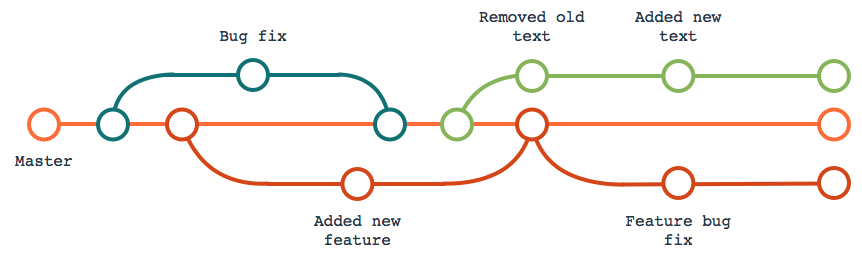
\includegraphics[scale=0.5]{./ressource/master_branche.png}
\end{center}

Un outil de versioning permet de maintenir, gérer les versions d'un ou plusieurs fichiers. Différents outils logiciels existent pour cela : 
\begin{itemize}
\itemE CVS
\itemE SVN 
\itemE Mercurial
\itemE \textbf{Git} (celui traité dans ce document)
\end{itemize}

\begin{center}

\includegraphics[scale=0.4]{./ressource/git_logo.png}
\end{center}

\section{Caractéristique de Git}
\begin{itemize}
\itemE Rapide ;
\itemE Travailler par branches
\itemE Complexe à prendre en mains 
\itemE Prévu pour Linux à l'origine
\end{itemize}

Lorsqu’on travaille avec Git, on suit les différentes étapes ci-dessous : 

\begin{enumerate}
\item on modifie un fichier
\item on teste si le programme pour vérifier si cela fonctionne
\item on fait un commit pour "enregistrer" les changements et les faire connaître à Git
\item et on recommence
\end{enumerate}


\vspace{0.5cm}


Git a trois grandes fonctionnalités :
\begin{itemize}
\itemE Revenir à une version précédente de votre code en cas de problème.
\itemE Suivre l’évolution de votre code étape par étape.
\itemE Travailler à plusieurs sans risquer de supprimer les modifications des autres collaborateurs. 
\end{itemize}

\begin{center}
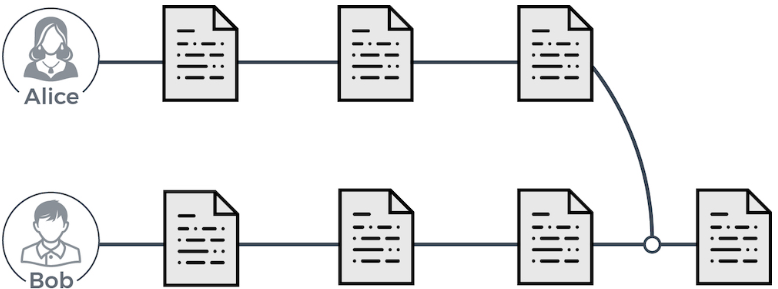
\includegraphics[scale=0.7]{./ressource/alice_bob_git.png}
\end{center}


\section{Fonctionnement de GIT}
\tiny Ref : Openclassroom \normalsize

Le Fonctionnement de GIT peut se résumer de la manière suivante ou chaque transition entre les états est définie par des commandes: 

\begin{center}
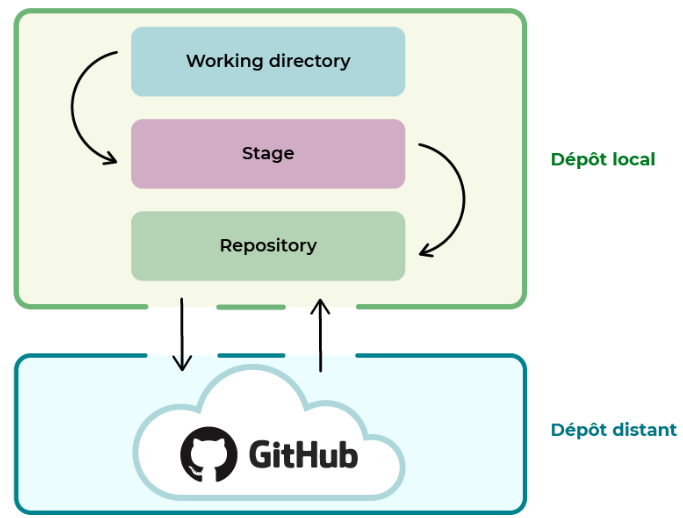
\includegraphics[scale=0.5]{./ressource/fctTGit}
\end{center}

\subsection{Dépôt local }

\begin{itemize}
\itemE \textbf{Working directory} : dossier contenant votre projet sur votre ordinateur
\itemE \textbf{Stage ou index} : Ensemble des fichiers modifiés que vous voulez voir apparaître dans la prochaine version
\itemE \textbf{Repository} : ensemble des différentes versions
\end{itemize}

\subsection{Dépôt distant}

C'est un lieux de stocakage sur le cloud ou chaque participant au projet va proposer ses modifications. L'ensemble des différentes versions est présent sur ce dépot. 
Le dépôt distant est donc un type de dépôt indispensable si vous travaillez à plusieurs sur le même projet, puisqu’il permet de centraliser le travail de chaque développeur. C’est aussi sur le dépôt distant que toutes les modifications de tous les collaborateurs seront fusionnées.

Plusieurs plateforme existent. Durant l'année, nous verrons : 

\begin{itemize}
\itemE \textbf{GitHub} : c'est un service web d'hébergement et de gestion de développement de logiciels, utilisant le logiciel de gestion de versions Git. Propriété de Microsoft, elle fait partie des platefrome les plus utilisé.
\end{itemize}

\begin{center}

\includegraphics[scale=0.1]{./ressource/gitLogo}
\end{center}

 Par exemple, beaucoup de librairie Arduino sont déposé sur GitHub. 
\begin{center}
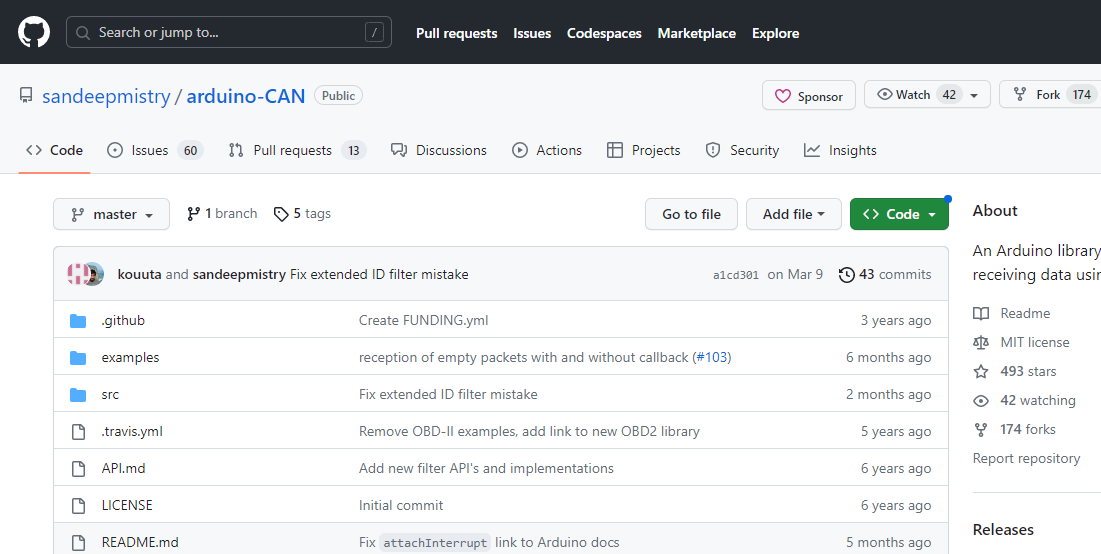
\includegraphics[scale=0.4]{./ressource/interfaceGitHub}
\end{center}


\begin{itemize}
\itemE \textbf{GitLab} est la principale alternatif à GitHub surtout depuis que Git Hub appartient à M\$ (principalement pour les pro logiciel libre et anti GAFAM). Le gros avantage de GitLab est de pouvoir créer vos propres serveurs.
\end{itemize}

\begin{center}

\includegraphics[scale=0.1]{./ressource/gitLab}
\end{center}


\section{Installation}

 \subsection{Sous Windows}
 
\begin{enumerate}
\item Allez sur le site de git et télécharger la version de git pour windows : \href{https://gitforwindows.org/}{Install Git}
\item Executer le fichier d'installation de git.
\item Lancer alors 	\verb?Git bash?

\begin{center}

\includegraphics[scale=0.7]{./ressource/gitbash}
\end{center}

\item Rentrer vos données personnelles 

\begin{lstlisting}[style=commande]
git config --global user.name "votreNom"
git config --global user.email "votreMail@mail.com"
\end{lstlisting}
\end{enumerate}


\subsection{Sous Linux}
\begin{enumerate}
\item Installer Git

\begin{lstlisting}[style=commande]
sudo apt install git 
\end{lstlisting}



\item Vérifier la version 

\begin{lstlisting}[style=commande]
git --version 
\end{lstlisting}


\item Rentrer vos données personnelles 

\begin{lstlisting}[style=commande]
git config --global user.name "votreNom"
git config --global user.email "votreMail@mail.com"
\end{lstlisting}


\end{enumerate}



\section{Commande pour un dépôt distant}
\begin{itemize}
\itemE git clone est utilisée pour la récupération des dépôts. Si le dépôt se trouve sur un serveur distant, il faut utiliser:
%%%%%%%%%%%%%%%%%%%%%%%%%%%%%%%%%%%%%%
\begin{lstlisting}[style=commande]
git clone addr_IP ou URL
\end{lstlisting}

\textbf{Cette commande est très importante elle permet de récupérer l'intégralité du dépôt sur la machine local.}


\vspace{0.5cm}

\itemE git push envoie les modifications locales apportées à la branche principale associée.
%%%%%%%%%%%%%%%%%%%%%%%%%%%%%%%%%%%%%%
\begin{lstlisting}[style=commande]
git push
\end{lstlisting}

\itemE Intègre les modifications d’un dépôt distant dans la branche actuelle.
\begin{lstlisting}[style=commande]
git pull
\end{lstlisting}

\itemE Git fetch permet de récupérer tous les fichiers du dépôt distant qui ne sont pas actuellement dans le répertoire de travail local.
%%%%%%%%%%%%%%%%%%%%%%%%%%%%%%%%%%%%%%
\begin{lstlisting}[style=commande]
git fetch
\end{lstlisting}

\itemE git request-push propose les modifications locales apportées à la branche principale associée.
%%%%%%%%%%%%%%%%%%%%%%%%%%%%%%%%%%%%%%
\begin{lstlisting}[style=commande]
git request-push
\end{lstlisting}


\end{itemize}

\section{Commandes de base en local}

\begin{itemize}
\itemE git add ajoute des fichiers à l’index (exemple : text.cpp)

%%%%%%%%%%%%%%%%%%%%%%%%%%%%%%%%%%%%%%
\begin{lstlisting}[style=commande]
git add text.cpp
\end{lstlisting}

\itemE git commit valider les modifications apportées. Il faut au préalable avoir effectuer une commande git add.	
%%%%%%%%%%%%%%%%%%%%%%%%%%%%%%%%%%%%%%
\begin{lstlisting}[style=commande]
git commit -m "Message relatif au commit"
\end{lstlisting}

\begin{center}
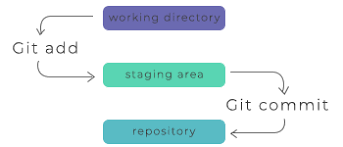
\includegraphics[scale=0.7]{./ressource/gitAddCommit}
\end{center}


\itemE  git status affiche la liste des fichiers modifiés ainsi que les fichiers qui doivent encore être ajoutés ou validés 	

%%%%%%%%%%%%%%%%%%%%%%%%%%%%%%%%%%%%%%
\begin{lstlisting}[style=commande]
git status
\end{lstlisting}


\itemE   git branch peut être utilisée pour répertorier, créer ou supprimer des branches 	
%%%%%%%%%%%%%%%%%%%%%%%%%%%%%%%%%%%%%%
\begin{lstlisting}[style=commande]
git branch 
\end{lstlisting}

%%%%%%%%%%%%%%%%%%%%%%%%%%%%%%%%%%%%%%
\begin{lstlisting}[style=commande]
git branch "nouvelle branche"
\end{lstlisting}

%%%%%%%%%%%%%%%%%%%%%%%%%%%%%%%%%%%%%%
\begin{lstlisting}[style=commande]
git branch -d "branche a supprimer"
\end{lstlisting}


\begin{center}
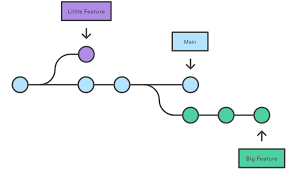
\includegraphics[scale=0.7]{./ressource/gitBranch}
\end{center}
\itemE git switch  peut-être utilisé pour passer d'une branche à une autre
\begin{lstlisting}[style=commande]
git switch "nom branche"
\end{lstlisting}



\itemE git checkout peut être utilisée pour basculer d'une version à une autre
%%%%%%%%%%%%%%%%%%%%%%%%%%%%%%%%%%%%%%
\begin{lstlisting}[style=commande]
git checkout "id du  commit"
\end{lstlisting}

\itemE git checkout peut être utilisée pour créer des branches à partir d'une version particulière
%%%%%%%%%%%%%%%%%%%%%%%%%%%%%%%%%%%%%%
\begin{lstlisting}[style=commande]
git checkout "id du  commit" -b  "nom_commit
\end{lstlisting}

\itemE git diff permet de lister les conflits
%%%%%%%%%%%%%%%%%%%%%%%%%%%%%%%%%%%%%%
\begin{lstlisting}[style=commande]
git diff 
\end{lstlisting}

\itemE git merge est utilisée pour fusionner une branche dans la branche active
%%%%%%%%%%%%%%%%%%%%%%%%%%%%%%%%%%%%%%
\begin{lstlisting}[style=commande]
git merge "nom branche"
\end{lstlisting}

\begin{center}
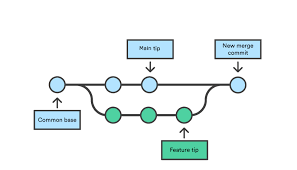
\includegraphics[scale=0.7]{./ressource/gitMerge}
\end{center}

\itemE git mergetool est utilisée pour régler les problèmes de conflit. En effet, lorsque l'on veut fusionner deux branches, si un ou des fichiers ont été simultanément modifiés dans deux branches, git refuse de réaliser le commit.  Pour résoudre le conflit, il faut lancer la commande suivante :
%%%%%%%%%%%%%%%%%%%%%%%%%%%%%%%%%%%%%%
\begin{lstlisting}[style=commande]
git mergetool "nom branche"
\end{lstlisting}

\begin{center}
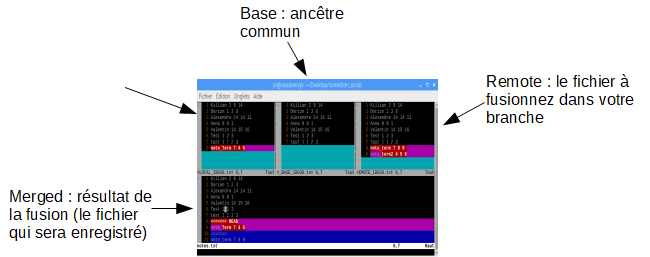
\includegraphics[scale=0.7]{./ressource/merge_tool.png}
\end{center}

Il suffit alors de ce déplacer avec le curseur dans la zone de conflit puis
\begin{itemize}
\item[+] ':diffg RE' pour prendre le modification de REMOTE
\item[+] ':diffg BA' pour prendre le modification de BASE
\item[+] ':diffg LO' pour prendre le modification de LOCAL
\end{itemize}

\itemE  git log génère le log d’une branche
%%%%%%%%%%%%%%%%%%%%%%%%%%%%%%%%%%%%%%
\begin{lstlisting}[style=commande]
git log
\end{lstlisting}

\itemE  git rm permet de déindexer des fichiers
%%%%%%%%%%%%%%%%%%%%%%%%%%%%%%%%%%%%%%
\begin{lstlisting}[style=commande]
git rm nomfichier.txt
\end{lstlisting}


\itemE Cette commande permet de visualiser l'arbre des commits avec ses différentes branches	
%%%%%%%%%%%%%%%%%%%%%%%%%%%%%%%%%%%%%%
\begin{lstlisting}[style=commande]
git log --oneline --graph --color --all --decorate
\end{lstlisting}

Ci-dessous un exemple d'arbre des commits.
\begin{center}
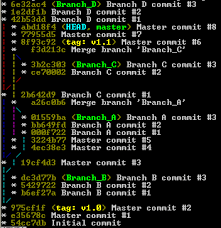
\includegraphics[scale=0.8]{./ressource/git_tree.png}
\end{center}

\end{itemize}



\section{Conclusion}

Vous avez découvert les principales commandes pour gérer les dépots GIT. Vous verrez toutes leurs puissances dans le reste des activités.


\end{document}
